\chapter{Merging calculus and dynamical systems}
\label{sec:calculus-and-physical-systems}

As said earlier, with the merge of calculus and trigonometry, all the cards are on the deck. This is all the calculus knowledge there is from here to the nineteenth-century.

\section{Further examples of calculus in physics and kinematics}

\subsection{Block sliding down a ramp with friction}

\begin{figure}[ht]
    \centering
    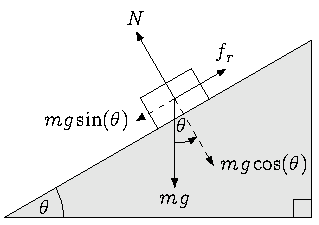
\includegraphics{geometricalsignificance/blockslidingdownaramp}
    \caption{A block sliding down a rough ramp (i.e. with friction) angled $\theta$ relative to the ground}
    \label{fig:blockslidingdownaramp}
\end{figure}
Illustrated in \cref{fig:blockslidingdownaramp}, there are two axis of motion: perpendicular and parallel to the block's expected motion. From what we know, there are the gravity $mg$ that pulls the block straight down and the friction force $f_r$ acting against the block's expected motion in the parallel axis. The problem constraints use along the perpendicular axis: the block can't move along that perpendicular axis \emph{because there's a ramp in the way}. Therefore, the ramp must act a force $N$ on the block.

We want to find the equation of motion for this block that's sliding down a ramp with friction. As far as the perpendicular axis goes, we don't have to worry about that one because nothing is moving there anyways. On the parallel axis, there's the $f_r$ and $mg\sin(\theta)$.\footnote{Just decompose $mg$ into its parallel and perpendicular axis. Using basic trigonometry is enough.} If we set the direction of the parallel axis to pointing downwards along the block's movement, we get that the total force is
\begin{equation*}
    F_{n} = mg\sin(\theta) - f_r\footnote{$F_n$ for $F_{\textrm{net}}$ or, total force.}.
\end{equation*}
By the Newton's second law,
\begin{align*}
    m\odv{t}(\odv{x}{t}) = mg\sin(\theta) - f_r \\
    \odv{t}(\odv{x}{t}) = g\sin(\theta) - \frac{f_r}{m}.
\end{align*}
$g\sin(\theta) - \flatfrac{f_r}{m}$ doesn't change with time, let's name it $\kappa$. The equation then becomes
\begin{align}
    \odv{t}(\odv{x}{t}) &= \kappa \label{eq:blockslidingdownarampaux}\\
    \int\odif(\odv{x}{t}) &= \int\kappa\odif{t} \nonumber\\
    \odv{x}{t} &= \kappa t \nonumber \\
    \int\odif{x} &= \int\kappa t\odif{t} \nonumber\\
    x(t) &= \left(g\sin(\theta) - \frac{f_r}{m}\right)\frac{t^2}{2}.
\end{align}
which \emph{is} our equation of motion. Notice, \cref{eq:blockslidingdownarampaux} literally has the same form as \cref{eq:accelerationfromgravity} that we derived from ``ball dropped from a building''. And indeed, it should be the same because it's just a thing that's under a constant acceleration. 

\subsection{One-dimensional movement with drag forces}

The free body diagram is illustrated in \cref{fig:projectileswithdragforce}. There's the gravity $m\vv{g}$ pulling the ball down, and drag force $kf_r(\vv{v})$. However, drag is a complex thing. There is no such thing as an ``exact drag function'' because drag depends on so many variables, e.g., air viscosity, air compressibility, object's shape, surface's friction, just to name a few. Therefore, the drag function $f_r(\vv{v})$ is a \emph{simplified model}, not the real thing.\index{drag function (simplified model)}

We shall model the drag based on two assumptions. \begin{enumerate*}[label = \roman*.)]
    \item the drag force should depend on the velocity : the faster, the more drag. And,
    \item any function can be approximated using the power series expansion (also discussed in \cref{sec:afunctionthatisitsownderivative}):
\end{enumerate*}
\begin{equation*}
    f_r(\vv{v}) = a_0 + a_1\vv{v} + a_2\vv{v}^2 + a_3\vv{v}^3 + \dots.
\end{equation*}
Considering only the first three terms should be enough. We know that $a_0$ must be $0$, because otherwise our object would just accelerate all the time, which is no good. Therefore, there can only be $a_1\vv{v} + a_2\vv{v}^2$. Newton's second law reads
\begin{equation*}
	m\odv*{(\odv{x}{t})}{t} = a_1\odv{x}{t} + a_2\ab(\odv{x}{t})^2.
\end{equation*}
Using fluxion notation,
\begin{align*}
    m\odv{\dot{x}}{t} &= a_1\dot{x} + a_2\dot{x}^2 \\
    \odv{\dot{x}}{t} &= \frac{a_1}{m}\dot{x} + \frac{a_2}{m}\dot{x}^2
\end{align*}
For convenience, let $\flatfrac{a_1}{m} = p$ and $\flatfrac{a_2}{m} = q$. The equation reads
\begin{equation}
    \odv{\dot{x}}{t} = p\dot{x} + q\dot{x}^2. \label{eq:quadraticdrageq}
\end{equation}

It is obvious that both $p$ and $q$ must be negative, otherwise the object would accelerate forward with the velocity. Frankly, \cref{eq:quadraticdrageq} is not possible to solve using the techniques that we have now. I'll revisit this exact differential equation later in \cref{eq:advtechniquesrationalfunctions}. For now, we shall deal with a simpler equation by considering two cases: only linear drag and only quadratic drag.

\subsubsection{Motion with just linear drag}

You don't really see linear drag in real life. It's mostly drag in moving liquid, e.g., a fish swimming in the water. \Cref{eq:quadraticdrageq} simplifies to
\begin{equation*}
    \odv{\dot{x}}{t} = p\dot{x}.
\end{equation*}
I shall set $v_0$ as the initial velocity and $x_0$ as the initial position. There are two methods of solving this. First, by separating variables using analytical methods.
\begin{align}
    \int\frac{1}{\dot{x}}\odif{\dot{x}} &= p\int\odif{t} \nonumber\\
    \ln(\dot{x}) + C &= pt. \label{eq:motionlineardrag1}
\end{align}
To find out what this integration constant should be, we have to use the initial condition $t = 0 \implies \dot{x} = v_0$.
\begin{align*}
    \ln(v_0) + C &= 0 \\
    C &= -\ln(v_0).
\end{align*}
\Cref{eq:motionlineardrag1} then becomes
\begin{align}
    \ln(\dot{x}) - \ln(v_0) &= pt \nonumber\\
    \dot{x} &= v_0\e^{pt}. \label{eq:motionlineardrag2}
\end{align}

\begin{figure}
    \centering
    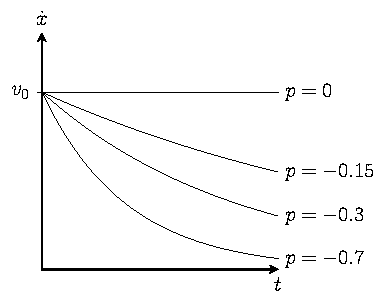
\includegraphics{geometricalsignificance/motionlineardragv}
    \caption{Plot of \cref{eq:motionlineardrag2} with various $p$.}
    \label{fig:motionlineardragv}
\end{figure}
\Cref{fig:motionlineardragv} plots \cref{eq:motionlineardrag2} with various $p$. Notice that when $p = 0$, \cref{eq:motionlineardrag2} is just a straight line $\dot{x} = v_0$. The more negative $p$ is, the faster it slows down, as illustrated. That is why sometimes, we call $p$ the \textbf{dampening factor}\index{dampening factor}. Also, $v_0$ here just scales the graph in the $\dot{x}$ direction.

To find $x(t)$, we rewrite \cref{eq:motionlineardrag2} as
\begin{equation*}
    \odv{x}{t} = v_0\e^{pt}.
\end{equation*}
Then,
\begin{align}
    \odif{x} &= v_0\e^{pt}\odif{t} \\
    x + C_1 &= v_0\int \e^{pt}\odif{t}. \label{eq:motionlineardrag3}
\end{align}

Here, I shall introduce an integration technique called \textbf{change of variables}\index{change of variables!naive}, commonly known as $u$-substitution. We'll formally come back to this topic later in \cref{sec:changeofvariables}. Basically, it's a way to convert integrals that we don't recognize into an easier integral. It's better if I just show the examples. We don't know the antiderivative of $\e^{pt}$ in \cref{eq:motionlineardrag3}, however we know the antiderivative of $\e^{u}$. So let's convert $\e^{pt}$ into that form. By letting a dummy variable $u = pt - v_0$, we have to convert $\odif{u}$ into $\odif{t}$ aswell.
\begin{align*}
    u &= pt - v_0 \\
	\odv{u}{t} &= \odv*{(pt - v_0)}{t} \\
    \frac{1}{p}\odif{u} &= \odif{t}.
\end{align*}
Then, substituting $\odif{t} = \frac{1}{p}\odif{u}$ and $u = pt$ into \cref{eq:motionlineardrag3}, it reads
\begin{align}
    x + C_1 &= v_0\int\e^{u}\ab(\frac{1}{p}\odif{u}) \nonumber\\
    x + C_1 &= \frac{v_0}{p}\e^{pt}. \label{eq:motionlineardrag4}
\end{align}

We also have to take care of the $C_1$. Using $t = 0 \implies x = x_0$,
\begin{align*}
    x_0 + C_1 &= \frac{v_0}{p}\e^{p\cdot(0)} \\
    C_1 &= \frac{v_0}{p} - x_0.
\end{align*}
Then, plug it into \cref{eq:motionlineardrag4}. The equation becomes
\begin{align}
    x + \frac{v_0}{p} - x_0 &= \frac{v_0}{p}(\e^{pt}) \nonumber\\
    x &= x_0 + \frac{v_0}{p}(\e^{pt} - 1). \label{eq:motionlineardrag5}
\end{align}

I've plotted \cref{eq:motionlineardrag5} with varying $v$ in \cref{fig:motionlineardragx1} and varying $p$ in \cref{fig:motionlineardragx2}. The graph should match with what you expect intuitively: higher $v$ will get you further, and the less the drag, the further you'll get.

\begin{figure}[ht]
    \centering
    \begin{subfigure}[l]{0.45\textwidth}
        \centering
        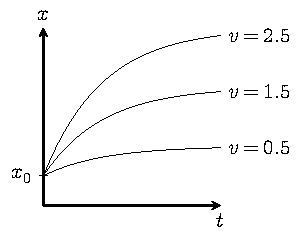
\includegraphics{geometricalsignificance/motionlineardragx1}
        \caption{with varying $v$, setting $p = -1$}
        \label{fig:motionlineardragx1}
    \end{subfigure}
    \begin{subfigure}[r]{0.45\textwidth}
        \centering
        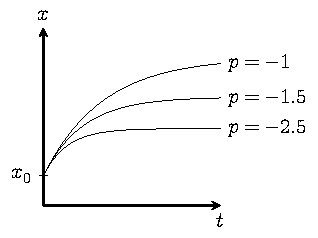
\includegraphics{geometricalsignificance/motionlineardragx2}
        \caption{with varying $p$, setting $v = 2$}
        \label{fig:motionlineardragx2}
    \end{subfigure}
    \caption{Plot of \cref{eq:motionlineardrag5}, setting $x_0 = 0.5$.}
\end{figure}

Notice, this motion has a clear upper limit. \emph{If $p \in \mathbb{R}^-$}, $\lim_{t \appr \infty}e^{pt} = 0$. Taking the limit as $t \appr 0$ on both sides of \cref{eq:motionlineardrag5}, we get
\begin{align*}
    \lim_{t \appr \infty} x(t) &= \lim_{t \appr \infty}\left(x_0 + \frac{v_0}{p}(e^{pt} - 1)\right). \\
    &= x_0 + \frac{v_0}{p}\cancelto{0}{\lim_{t \appr 0}\left(e^{pt}\right)} - \frac{v_0}{p} = x_0 - \frac{v_0}{p},
\end{align*}
which when $p \in \mathbb{R}^-$ and $v_0\in\mathbb{R}^+$, the motion procedes forward, then gradually slows down and stops at $x_0 - \frac{v_0}{p}$ which is more than $x_0$.

\subsubsection{Motion with just quadratic drag}

\begin{multicols}{2}
This equation is even easier than linear drag, so I'd leave out some steps. \Cref{eq:quadraticdrageq} simplifies to
\begin{align*}
    \odv{\dot{x}}{t} &= q\dot{x}^2 \\
    \int \frac{1}{\dot{x}^2}\odif{\dot{x}} &= q\int\odif{t} \footnote{Hint: $\flatfrac{1}{\dot{x}^2} = \dot{x}^{-2}$}\\
    - \frac{1}{\dot{x}} + C = qt.
\end{align*}
Taking care of $C$: use $t = 0 \implies \dot{x} = v_0$.
\begin{align*}
    - \frac{1}{v_0} + C &= q\cdot 0 \\
    C &= \frac{1}{v_0}.
\end{align*}
Therefore,
\begin{align}
    -\frac{1}{\dot{x}} + \frac{1}{v_0} &= qt \nonumber\\
    \odv{t}{x} &= \frac{1 - qv_0t}{v_0} \nonumber\\
    x &= v_0\int\frac{1}{1 - qv_0t} \odif{t}. \label{eq:motionquadraticdrag1}
\end{align}
The structure of the integral is similar to $\flatfrac{1}{t}$. Therefore, let $u = 1 - qv_0t$. Then,
\begin{align*}
    \odv{u}{u} &= \odif{u}(1 - qv_0t) \\
    1 &= -qv_0\odv{t}{u} \\
    \odif{t} &= -\frac{1}{qv_0}\odif{u}.
\end{align*}
Substitute $u = 1 - qv_0t$ and $\odif{t} = -\frac{1}{qv_0}\odif{u}$ into \cref{eq:motionquadraticdrag1}:
\begin{align}
    x &= v_0 \int \frac{1}{u}\left(-\frac{1}{qv_0}\odif{u}\right) \nonumber\\
    &= -\frac{1}{q}\int \frac{1}{u}\odif{u} \nonumber\\
    x(t) &= -\frac{1}{q}\ln(1 - qv_0t) + C_1. \label{eq:motionquadraticdrag2}
\end{align}
Taking care of $C_1$: use $t \appr 0 \implies x(t) = x_0$.
\begin{align*}
    x_0 &= -\frac{1}{q}\ln(1 - qv_0\cdot(0)) + C_1 \\
    x_0 &= C_1
\end{align*}
Plug this into \cref{eq:motionquadraticdrag2} to get the final answer:
\begin{equation*}
    x(t) = -\frac{1}{q}\ln(1 - qv_0t) + x_0.
\end{equation*}
\end{multicols}

Surprisingly, quadratic drag does not have upper position bounds. A bit more thought would reveal that when $v < 0$, the quadratic drag $f_r(v) = a_2v^2$ is smaller thasecn $f_r(v) = a_1v$. Thus, it should makes sense that quadratic doesn't have bounds, but linear has an upper bound.

\subsubsection{Terminal velocity of objects}

\subsection{Time of meteor collision from great height}

Illustrated in \cref{fig:meteorfallingfromgreatheight}\footnote{Not to scale.}, a meteor is falling from height $h$ above the Earth. Let's find the time that it'd take to hit the Earth.
\begin{figure}[ht]
    \centering
    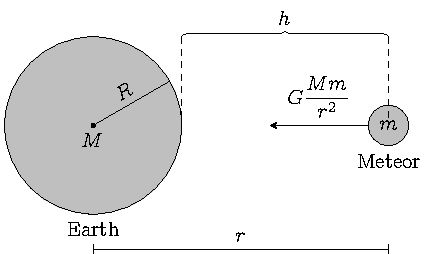
\includegraphics{geometricalsignificance/meteorfallingfromgreatheight}
    \caption{An illustration of a meteor falling to the Earth from height $h$.}
    \label{fig:meteorfallingfromgreatheight}
\end{figure}
The meteor has the mass $m$, falling from height $h$ above the ground. The Earth has mass $M$, radius $R$. Let's denote the meteor's position relative to the Earth's center with $r$. The initial condition of the meteor is $r(0) = h + R$, and $\dot{r}(0) = v_0$ For simplicity sake, let the meteor be a mass point: its radius is zero, and the Earth is very massive compared to the meteor so it doesn't move with the meteor's gravitational attraction. Given by Newton's law of gravitational attraction, the Earth is pulling the meteor by
\begin{equation*}
    F = G\frac{Mm}{r^2}.
\end{equation*}
Therefore, Newton's second law on the meteor reads
\begin{equation*}
	G\frac{Mm}{r^2} = m\odv*{\ab(\odv{r}{t})}{t}\footnote{Notice that here, $r$ also changes with time.}.
\end{equation*}

To frame the problem mathematically, we want to find an equation of motion of the meteor. Then, find the time it takes for the meteor to travel from $h + R$ (initial position) to $R$ (the ground).

The $m$ on both sides cancel. For convenience, let $\kappa = GM$
\begin{equation}
    \frac{\kappa}{r^2} = \odv{\dot{r}}{t}. \label{eq:meteorfallingfromgreatheight1}
\end{equation}
Solving this equation is not at all trivial: there are \emph{three} variables, i.e., $r$. $\dot{r}$, and $t$; however, an equation only has two sides. We can't possibly separate these variables. Here, I shall introduce a technique for solving this kind of differential equation. With the chain rule,
\begin{equation*}
    \odv{\dot{r}}{t} = \odv{\dot{r}}{r} \cdot \odv{r}{t} = \dot{r}\odv{\dot{r}}{r}:
\end{equation*}
we converted an expression that's dependent on other variable $t$ to be dependent on a lower derivative $r$ instead! Then $t$ is removed, or rather, hidden. You can interpret $\odv*{\dot{r}}{r}$ as the velocity at any given distance away from the Earth. Plug this into \cref{eq:meteorfallingfromgreatheight1}, we get
\begin{align}
    \frac{\kappa}{r^2} &= \dot{r}\odv{\dot{r}}{r} \nonumber\\
    \kappa\int\frac{1}{r^2}\odif{r} &= \int\dot{r}\odif{\dot{r}} \nonumber\\
    \frac{\kappa}{r} + C &= \frac{\dot{r}^2}{2} \label{eq:meteorfallingfromgreatheight2}
\end{align}
The term $+C$ is going to be a different because now, we don't have a $t$ to fix our initial condition. However, we know that when $\dot{r} = v_0$, $r = h + R$. Therefore,
\begin{align*}
    -\frac{\kappa}{h + R} + C &= \frac{v_0^2}{2} \\
    C &= \frac{v_0^2}{2} - \frac{\kappa}{r}.
\end{align*}
However, the structure of $C$ is quite complicated so, I wouldn't substitute it in yet until we get our final answer. Continuing with \cref{eq:meteorfallingfromgreatheight2}, we turn the $\dot{r}$ into the Leibniz's notation:
\begin{align*}
    \frac{\kappa + Cr}{r} &= \frac{1}{2}\left(\odv{r}{t}\right)^2. \\
    \sqrt{2}\sqrt{\frac{\kappa + Cr}{r}} &= \odv{r}{t} \\
    \int\odif{t} &= \sqrt{2}\int\sqrt{\frac{r}{\kappa + Cr}}\odif{r}
\end{align*}

Unfortunately, this integral is very hard to solve. But it is possible, and the solution to this integral is
\begin{equation*}
    \frac{C}{\kappa^{\flatfrac{3}{2}}\sqrt{r}}\sqrt{\frac{r}{\kappa r + C}}\sqrt{\frac{\kappa r}{C} + 1} \left(\sqrt{\kappa r}\sqrt{\frac{\kappa r}{C} + 1} - \sqrt{C}\sinh^{-1}\left(\sqrt{\frac{\kappa x}{C}}\right)\right),
\end{equation*}
which is quite a nightmare, but we will get back to this in the far far future.

\subsection{Damped harmonic motion}

\section{Conservation laws}
